\section{CÔNG THỨC NHÂN XÁC SUẤT}
\subsection{LÝ THUYẾT CẦN NHỚ}
\subsubsection{BIẾN CỐ ĐỘC LẬP}
\begin{enumerate}[\iconMT]
	\item \indam{Định nghĩa:} Cho hai biến cố $A$ và $B$. Hai biến cố $A$ và $B$ được gọi là độc lập nếu việc xảy ra hay không xảy ra của biến cố này không làm ảnh hưởng đến xác suất xảy ra của biến cố kia.
	\item \indam{Chú ý:} Nếu $A, B$ là hai biến cố độc lập thì mỗi cặp biến cố sau cũng độc lập: $A$ và $\overline{B} ; \overline{A}$ và $B ; \overline{A}$ và $\overline{B}$.
\end{enumerate}
\subsubsection{CÔNG THỨC NHÂN XÁC SUẤT}

Nếu hai biến cố $A$ và $B$ là độc lập thì \boxmini{$\mathrm{P}(A B)=\mathrm{P}(A) . \mathrm{P}(B)$}
\begin{luuy}
	Nếu $\mathrm{P}(A B)\ne \mathrm{P}(A) . \mathrm{P}(B)$ thì $A$ và $B$ không độc lập.
\end{luuy}


\subsection{PHÂN LOẠI VÀ PHƯƠNG PHÁP GIẢI TOÁN}

\begin{dang}{Biến cố độc lập}
\end{dang}

\begin{vd}%[1D2B2-4]
	Gieo hai đồng xu cân đối. Xét các biến cố $A$: \lq\lq Cả hai đồng xu đều ra mặt sấp\rq\rq, $B$: \lq\lq Có ít nhất một đồng xu ra mặt sấp\rq\rq. Hỏi $A$ và $B$ có độc lập hay không?
	\loigiai{
		Ta có $\Omega=\left\lbrace SS; SN; NS; NN\right\rbrace $. Do đó $\mathrm{n}\left(\Omega \right)=4$, $A=\left\lbrace SS \right\rbrace, \mathrm{n}\left(A \right)=1$. Vậy $\mathrm{P}\left(A\right)=\dfrac{1}{4}$.\\
		Ta có $B=\left\lbrace SS; SN; NS\right\rbrace $. Do đó $\mathrm{n}\left(B \right)=3$. Vậy $\mathrm{P}\left(B\right)=\dfrac{3}{4}$.\\
		Ta có $AB=A\cap B=\left\lbrace SS \right\rbrace  $. Do đó $\mathrm{n}\left(A\cap B \right)=1$. Vậy $\mathrm{P}\left(AB\right)=\dfrac{1}{4}$.\\
		Ta có $\mathrm{P}\left(AB\right)=\dfrac{1}{4}=\dfrac{4}{16}\neq \mathrm{P}\left(A \right)\cdot \mathrm{P}\left(B \right)=\dfrac{1}{3}\cdot \dfrac{3}{4}=\dfrac{3}{16}$.\\
		Vậy $A$ và $B$ không độc lập      	
	}
\end{vd}\dongcham{17}

\begin{vd}%[1K8KR-3]
	Một hộp đựng $4$ viên bi màu đỏ và $5$ viên bi màu xanh, có cùng kích thước và khối lượng.
	\begin{enumerate}
		\item Bạn Minh lấy ngẫu nhiên một viên bi, ghi lại màu của viên bi được lấy ra rồi trả lại viên bi vào hộp. Tiếp theo, bạn Hùng lấy ngẫu nhiên một viên bi từ hộp đó. Xét hai biến cố sau:\\	
		$A$: \lq\lq Minh lấy được viên bi màu đỏ\rq\rq;\\	
		$B$: \lq\lq Hùng lấy được viên bi màu xanh\rq\rq.\\	
		Chứng tỏ rằng hai biến cố $A$ và $B$ độc lập.
		\item Bạn Sơn lấy ngẫu nhiên một viên bi và không trả lại vào hộp. Tiếp theo, bạn Tùng lấy ngẫu nhiên một viên bi từ hộp đó. Xét hai biến cố sau:\\	
		$C$: \lq\lq Sơn lấy được viên bi màu đỏ\rq\rq;\\	
		$D$: \lq\lq Tùng lấy được viên bi màu xanh\rq\rq.\\	
		Chứng tỏ rằng hai biến cố $C$ và $D$ không độc lập.
	\end{enumerate}
	\loigiai{
		\begin{enumerate}
			\item Nếu $A$ xảy ra, tức là Minh lấy được viên bi màu đỏ. Vì Minh trả lại viên bi đã lấy vào hộp nên trong hộp có $4$ viên bi màu đỏ và $5$ viên bi màu xanh. Vậy $P(B)=\dfrac{5}{9}$.\\	
			Nếu $A$ không xảy ra, tức là Minh lấy được viên bi màu xanh. Vì Minh trả lại viên bi đã lấy vào hộp nên trong hộp vẫn có $4$ viên bi màu đỏ và $5$ viên bi màu xanh. Vậy $P(B)=\dfrac{5}{9}$.\\	
			Như vậy, xác suất xảy ra của biến cố $B$ không thay đổi bởi việc xảy ra hay không xảy ra của biến cố $A$.\\	
			Vì Hùng lấy sau Minh nên $P(A)=\dfrac{4}{9}$ dù biến cố $B$ xảy ra hay không xảy ra.\\	
			Vậy $A$ và $B$ độc lập.
			\item Nếu $C$ xảy ra, tức là Sơn lấy được viên bi màu đỏ. Vì Sơn không trả lại viên bi đó vào hộp nên trong hộp có $8$ viên bi với $3$ viên bi màu đỏ và $5$ viên bi màu xanh. Vậy $P(D)=\dfrac{5}{8}$. \\
			Nếu $C$ không xảy ra, tức là Sơn lấy được viên bi màu xanh. Vì Sơn không trả lại viên bi đã lấy vào hộp nên trong hộp có $4$ viên bi màu đỏ và $4$ viên bi màu xanh. Vậy $P(D)=\dfrac{4}{8}$. \\
			Như vậy, xác suất xảy ra của biến cố $D$ đã thay đổi phụ thuộc vào việc biến cố $C$ xảy ra hay không xảy ra. Do đó, hai biến cố $C$ và $D$ không độc lập.
		\end{enumerate}
	}
\end{vd}

\dongcham{13}

\begin{dang}{Công thức nhân xác suất của hai biến cố độc lập}
\end{dang}


\begin{vd}%[1D2B2-6]
	Cho hai biến cố độc lập $A$ và $B$ cùng liên quan đến một phép thử thỏa mãn $\mathrm{P}(A)=0{,}2$ và $\mathrm{P}(B)=0{,}3$. Tính xác suất của các biến cố: $\overline{A}$, $\overline{B}$, $AB$, $\overline{A} B$, $A \overline{B}$ và $\overline{A}\overline{B}$.
	\loigiai{
		$P(\overline{A})=1-P(A)=1-0{,}2=0{,}8$;\\
		$P(\overline{B})=1-P(B)=1-0{,}3=0{,}7$;\\
		$A$ và $B$ là hai biến cố độc lập nên các cặp biến cố sau cũng độc lập: $\overline{A}$ và $B$, $A$ và $\overline{B}$, $\overline{A}$ và $\overline{B}$.\\
		Ta có $P(A\cap B)=P(A)\cdot P(B)=0{,}2\cdot 0{,}3=0{,}06$.\\
		Tương tự ta có $P(\overline{A}\cap B)=0{,}24$; $P(A\cap \overline{B})=0{,}14$; $P(\overline{A}\cap \overline{B})=0{,}56$.
	}
\end{vd}\dongcham{12}



\begin{vd}%[1D2K2-6]
	Hai bệnh nhân cùng nhiễm một loại virus. Xác suất biến chứng nặng của bệnh nhân thứ nhất và bệnh nhân thứ hai lần lượt là $0{,}2$ và $0{,}25$; khả năng bị biến chứng nặng của hai bệnh nhân là độc lập. Tính xác suất của các biến cố:
	\begin{tasks}
		\task $M\colon$ \lq\lq Bệnh nhân thứ nhất và bệnh nhân thứ hai đều bị biến chứng nặng\rq\rq;
		\task $N\colon$ \lq\lq Bệnh nhân thứ nhất không bị biến chứng nặng và bệnh nhân thứ hai bị biến chứng nặng\rq\rq;
		\task $Q\colon$ \lq\lq Bệnh nhân thứ nhất bị biến chứng nặng và bệnh nhân thứ hai không bị biến chứng nặng\rq\rq;
		\task $R\colon$ \lq\lq Bệnh nhân thứ nhất và bệnh nhân thứ hai đều không bị biến chứng nặng\rq\rq;
		\task $S\colon$ \lq\lq Có ít nhất một trong hai bệnh nhân bị biến chứng nặng\rq\rq.
	\end{tasks}
	\loigiai{
		Xét hai biến cố: 
		\begin{itemize}
			\item $A\colon$ \lq\lq Bệnh nhân thứ nhất bị biến chứng nặng\rq\rq;
			\item $B\colon$ \lq\lq Bệnh nhân thứ hai bị biến chứng nặng\rq\rq.
		\end{itemize}
		$A$ và $B$ là hai biến cố độc lập, $n(A)=0{,}2$; $n(B)=0{,}25$.
		\begin{enumerate}[a)]
			\item $P(M)=P(A\cap B)=0{,}2\cdot 0{,}25=0{,}05$.
			\item $P(N)=P(\bar{A}\cap B)=0{,}8\cdot 0{,}25=0{,}2$.
			\item $P(Q)=P(A\cap \bar{B})=0{,}2\cdot 0{,}75=0{,}15$.
			\item $P(R)=P(\bar{A}\cap \bar{B})=0{,}8\cdot 0{,}75=0{,}6$.
			\item $P(S)=1-P(R)=1-0{,}6=0{,}4$.
		\end{enumerate}
	}
\end{vd}\dongcham{18}


\begin{vd}
	Có hai hộp chứa các quả cầu. Hộp thứ nhất  chứa $ 7 $ quả cầu màu đỏ và $ 5 $ quả cầu màu xanh; hộp thứ hai chứa $ 6 $ quả cầu màu đỏ và $ 4 $ quả cầu màu xanh. Lấy ngẫu nhiên từ mỗi hộp $ 1 $ quả cầu. Tính xác suất sao cho hai quả cầu lấy ra cùng màu đỏ.
	\loigiai{
		Xác suất lấy được quả cầu đỏ từ hộp 1: $ \mathrm{P_1} = \dfrac{7}{12} $.\\[5pt]
		Xác suất lấy được quả cầu đỏ từ hộp 2: $ \mathrm{P_2} = \dfrac{6}{10} $.\\
		Xác suất cần tìm $ \mathrm{P} = \mathrm{P_1}\mathrm{P_2} = \dfrac{7}{20}  $.
	}
\end{vd}\dongcham{9}

\begin{vd}
	Một phần mềm chuyển đổi ngôn ngữ có xác suất dịch chính xác một câu Tiếng Anh sang Tiếng Việt là $0{,}8$. Hỏi nếu phần mềm đó dịch một văn bản $100$ câu từ Tiếng Anh sang Tiếng Việt thì xác suất dịch sai hai câu là bao nhiêu?
	\loigiai{
		Xác suất để dịch chính xác một câu Tiếng Anh sang Tiếng Việt là $0{,}8$ và dịch sai một câu là $1-0{,}8=0{,}2$.\\
		Số cách chọn ra 2 câu dịch sai trong $100$ câu là $\mathrm{C}_{100}^{2}$.\\
		Suy ra, xác suất để dịch một văn bản $100$ câu từ Tiếng Anh sang Tiếng Việt thì xác suất dịch sai hai câu là
		$$\mathrm{P}=\mathrm{C}_{100}^{2}\left(0{,}2 \right)^{2}\cdot\left(0{,}8 \right)^{98}\approx 0{,}00000006302.  $$
	}
\end{vd}\dongcham{16}
\begin{vd}%[1D2B2-5]
	Hai bạn An và Bình cùng tập ném bóng rổ một cách độc lập ở hai nửa sân khác nhau. Xác suất bạn An và bạn Bình ném bóng vào rổ lần lượt là $0,6$ và $0,9$. Trong cùng một lần ném, tính xác suất có ít nhất một bạn ném bóng vào rổ.
	\loigiai{
		Xét các biến cố $A$: \lq\lq Bạn An ném bóng trúng rổ\rq\rq;
		$B$: \lq\lq Bạn Bình ném bóng trúng rổ\rq\rq;
		$C$: \lq\lq Có ít nhất một bạn ném bóng vào rổ\rq\rq.\\
		$A$ và $B$ là hai biến cố độc lập nên $\mathrm{P}\left(A\cap B\right)=\mathrm{P}\left(A\right)\cdot \mathrm{P}\left(B\right)$.\\
		Khi đó $\mathrm{P}\left(C\right)=\mathrm{P}\left(A\cup B\right)=\mathrm{P}\left(A\right)+\mathrm{P}\left(B\right)-\mathrm{P}\left(B\right)\cdot \mathrm{P}\left(C\right)=0,6+0,9-0,6\cdot 0,9=0,96$.}
\end{vd}\dongcham{19}

\begin{vd}%[1D2B2-4]
	Hai bạn An và Bình không quen biết nhau và đều học xa nhà. Xác suất để bạn An về thăm nhà vào ngày Chủ nhật là $0{,}2$ và của bạn Bình là $0{,}25$. Dùng sơ đồ hình cây để tính xác suất vào ngày Chủ nhật mà
	\begin{listEX}[2]
		\item cả hai bạn đều về thăm nhà.
		\item có ít nhất một bạn về thăm nhà.
		\item cả hai bạn đều không về thăm nhà.
		\item Chỉ có bạn An về thăm nhà.
		\item có đúng một bạn về thăm nhà.
	\end{listEX}
	\loigiai{
		Gọi $A$, $B$ tương ứng là các biến cố: ``Bạn An về thăm nhà vào ngày Chủ nhật'' và ``Bạn Bình về thăm nhà vào ngày Chủ nhật''. $A$ và $B$ là hai biến cố độc lập. Ta có sơ đồ hình cây:
		\begin{center}
			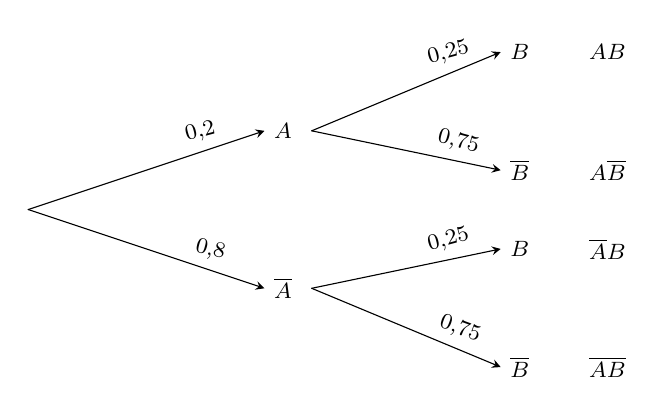
\begin{tikzpicture}[line join=round,line cap=round, font=\footnotesize,scale=1,>=stealth]
				\draw[-stealth](0,0)--(3,1)node[above, near end,,rotate=15]{$0{,}2$}node[right]{$A$};	
				\draw[-stealth](3.6,1)--(6,2)node[above, near end,,rotate=15]{$0{,}25$}node[right]{$B$};
				\draw(7,2)node[right]{$AB$};
				\draw[-stealth](3.6,1)--(6,0.5)node[above, near end,,rotate=-15]{$0{,}75$}node[right]{$\overline{B}$};
				\draw(7,0.5)node[right]{$A\overline{B}$};
				\draw[-stealth](0,0)--(3,-1)node[above, near end,,rotate=-15]{$0{,}8$}node[right]{$\overline{A}$};
				\draw[-stealth](3.6,-1)--(6,-0.5)node[above, near end,,rotate=15]{$0{,}25$}node[right]{$B$};
				\draw(7,-0.5)node[right]{$\overline{A}B$};
				\draw[-stealth](3.6,-1)--(6,-2)node[above, near end,,rotate=-20]{$0{,}75$}node[right]{$\overline{B}$};
				\draw(7,-2)node[right]{$\overline{A}\overline{B}$};
			\end{tikzpicture}	
		\end{center}
		\begin{listEX}
			\item $\mathrm{P}(AB)=0{,}2 \cdot 0{,}25=0{,}05$.
			\item $\mathrm{P}(A \cup B)=\mathrm{P}(A)+\mathrm{P}(B)-\mathrm{P}(AB)=0{,}2+0{,}25-0{,}05=0{,}4$.
			\item $\mathrm{P}\left(\overline{A}\overline{B}\right)=0{,}8 \cdot 0{,}75=0{,}6$.
			\item $\mathrm{P}\left(A \overline{B}\right)=0{,}2 \cdot 0{,}75=0{,}15$.
			\item $\mathrm{P}\left(A \overline{B} \cup \overline{A} B\right)=\mathrm{P}\left(A\overline{B}\right)+\mathrm{P}\left(\overline{A} B\right)=0{,}2 \cdot 0{,}75+0{,}8 \cdot 0{,}25=0{,}35$.
		\end{listEX}
	}
\end{vd}\dongcham{18}
\subsection{BÀI TẬP TỰ LUYỆN}

\begin{baitap}%[1K8KR-3]
	Có hai chuồng nuôi thỏ. Chuồng I có $5$ con thỏ đen và $10$ con thỏ trắng. Chuồng II có $3$ con thỏ trắng và $7$ con thỏ đen. Từ mỗi chuồng bắt ngẫu nhiên ra một con thỏ. Xét hai biến cố sau:\\
	$A$: \lq\lq Bắt được con thỏ trắng từ chuồng I\rq\rq;\\
	$B$: \lq\lq Bắt được con thỏ đen từ chuồng Il\rq\rq.\\
	Chứng tỏ rằng hai biến cố $A$ và $B$ độc lập.
	\loigiai{
		Nếu $A$ xảy ra, tức là bắt được con thỏ trắng ở chuồng I. Khi đó, số thỏ ở chuồng II không bị thay đổi và có $3$ thỏ trắng và $7$ thỏ đen. Vậy $P(B)=\dfrac{7}{10}$.\\	
		Nếu $A$ không xảy ra, tức là bắt được thỏ đen ở chuồng I.Khi đó, số thỏ ở chuồng II không bị thay đổi và có $3$ thỏ trắng và $7$ thỏ đen. Vậy $P(B)=\dfrac{7}{10}$.\\	
		Như vậy, xác suất xảy ra của biến cố $B$ không thay đổi bởi việc xảy ra hay không xảy ra của biến cố $A$.\\	
		Tương tự $P(A)=\dfrac{2}{3}$ dù biến cố $B$ xảy ra hay không xảy ra.\\	
		Vậy $A$ và $B$ độc lập.
	}
\end{baitap}

\begin{baitap}%[1K8KR-3]
	Có hai chuồng nuôi gà. Chuồng I có $9$ con gà mái và $3$ con gà trống. Chuồng II có $3$ con gà mái và $6$ con gà trống. Bắt ngẫu nhiên một con gà của chuồng I để đem bán rồi dồn các con gà còn lại của chuồng I vào chuồng II. Sau đó bắt ngẫu nhiên một con gà của chuồng II. Xét hai biến cố sau:\\
	$E$: \lq\lq Bắt được con gà trống từ chuồng I\rq\rq;\\
	$F$: \lq\lq Bắt được con gà mái từ chuồng II\rq\rq.\\
	Chứng tỏ rằng hai biến cố $E$ và $F$ không độc lập.
	\loigiai{
		Nếu $E$ xảy ra, tức là bắt được con gà trống từ chuồng I. Vì con gà trống bị bắt đem đi bán và số gà ở chuồng I dồn vô chuồng II, nên khi bắt gà mái từ chuồng II sẽ có $12$ gà mái và $8$ gà trống. Vậy $P(F)=\dfrac{12}{20}=\dfrac{3}{5}$. \\
		Nếu $E$ không xảy ra, tức là bắt được con gà mái từ chuồng I. Vì con gà mái bị bắt đem đi bán và số gà ở chuồng I dồn vô chuồng II, nên khi bắt gà mái từ chuồng II sẽ có $11$ gà mái và $9$ gà trống. Vậy $P(F)=\dfrac{11}{20}$. \\
		Như vậy, xác suất xảy ra của biến cố $F$ đã thay đổi phụ thuộc vào việc biến cố $E$ xảy ra hay không xảy ra. Do đó, hai biến cố $E$ và $F$ không độc lập.
	}
\end{baitap}
\begin{baitap}%[1D2B2-4]
	Cho $\mathrm{P}\left(A \right)=0{,}4$; $\mathrm{P}\left(B \right)=0{,}5$; $\mathrm{P}\left( A\cup B \right)=0{,}6$. Hỏi $A$ và $B$ có độc lập hay không?
	\loigiai{
		$\mathrm{P}\left( AB\right) =\mathrm{P}\left(A \right)+\mathrm{P}\left( B\right)-\mathrm{P}\left( A\cup B \right)=0{,}3\neq \mathrm{P}\left(A \right)\cdot \mathrm{P}\left(B \right)=0{,}2$.\\ Vậy $A$ và $B$ không độc lập.
	}
\end{baitap} \cham{10}

\begin{baitap}%[1D2B2-4]
	Gieo hai con xúc xắc cân đối. Xét các biến cố:\\
	$A$: ``Có ít nhất một con xúc xắc xuất hiện mặt $5$ chấm'';\\
	$B$: ``Tổng số chấm xuất hiện trên hai con xúc xắc bằng $7$''.\\
	Chứng tỏ rằng $A$ và $B$ không độc lập.
	\loigiai{
		Tính $\mathrm{P}(A)$.\\
		Xét biến cố đối $\overline{A}$: ``Cả hai con xúc xắc không xuất hiện mặt $5$ chấm''.\\
		$\overline{A}=\{(a,b)\colon a,b \in\{1;2;3;4;6\}\}$.\\
		Ta có $\mathrm{n}\left(\overline{A}\right)=25$; $\mathrm{n}(\Omega)=36$.\\
		Vậy $\mathrm{P}\left(\overline{A}\right)=\dfrac{25}{36}$, do đó $\mathrm{P}(A)=1-\dfrac{25}{36}=\dfrac{11}{36}$.\\
		Tính $\mathrm{P}(B)$.\\
		Ta có $B=\{(1,6);(2,5);(3,4);(4,3);(5,2);(6,1)\}$, $\mathrm{n}(B)=6$.\\
		Vậy $\mathrm{P}(B)=\dfrac{6}{36}$.\\
		Tính $\mathrm{P}(AB)$.\\
		Ta có $AB=A \cap B=\{(2,5) ;(5,2)\}$, $\mathrm{n}(A \cap B)=2$.\\
		Vậy $\mathrm{P}(AB)=\dfrac{2}{36}$.\\
		Ta có $\mathrm{P}(AB)=\dfrac{2}{36}=\dfrac{72}{36^2}$; $\mathrm{P}(A) \cdot \mathrm{P}(B)=\dfrac{11}{36} \cdot \dfrac{6}{36}=\dfrac{66}{36^2}$.\\
		Suy ra $\mathrm{P}(AB) \neq \mathrm{P}(A) \cdot \mathrm{P}(B)$.\\
		Vậy $A$ và $B$ không độc lập.
	}
\end{baitap} \cham{10}

\begin{baitap}%[1D2B2-4]
	Có $3$ hộp I, II, III. Mỗi hộp chứa ba tấm thẻ đánh số $1,2,3$. Từ mỗi hộp rút ngẫu nhiên một tấm thẻ. Xét các biến cố sau:\\
	$A$: ``Tổng các số ghi trên ba tấm thẻ là $6$'';\\
	$B$: ``Ba tấm thẻ có ghi số bằng nhau''.
	\begin{listEX}
		\item Tính $\mathrm{P}(A), \mathrm{P}(B)$.
		\item Hỏi $A$, $B$ có độc lập không?
	\end{listEX}
	\loigiai{
		Ta có $\Omega=\{(a,b,c)\colon 1 \leq a,b,c \leq 3\}$, $\mathrm{n}(\Omega)=27$.
		\begin{listEX}
			\item Tinh $\mathrm{P}(A)$.\\
			$A=\{(1,2,3);(2,1,3);(3,1,2);(1,3,2);(3,2,1);(2,3,1);(2,2,2)\}$, $\mathrm{n}(A)=7$.\\
			Suy ra $\mathrm{P}(A)=\dfrac{7}{27}$.\\
			Tinh $\mathrm{P}(B)$.\\
			$B=\{(1,1,1) ;(2,2,2) ;(3,3,3)\}, \mathrm{n}(B)=3$. Suy ra $\mathrm{P}(B)=\dfrac{3}{27}$.
			\item Tính $\mathrm{P}(AB)$.\\
			Ta có $A \cap B=\{(2,2,2)\}$. Vậy $P(AB)=\dfrac{1}{27}$.\\
			Vì $\mathrm{P}(AB)=\dfrac{1}{27}=\dfrac{27}{27^2} \neq \dfrac{21}{27^2}=\dfrac{7}{27} \cdot \dfrac{3}{27}=\mathrm{P}(A) \cdot \mathrm{P}(B)$ nên $A$ và $B$ không độc lập.
		\end{listEX}
	}
\end{baitap} \cham{10}


\begin{baitap}%[1D2B2-5]
	Cho $A$ và $B$ là hai biến cố độc lập với nhau.
	\begin{enumerate}
		\item Biết $\mathrm{P}(A)=0,4$ và $\mathrm{P}(\overline{A} B)=0,3$. Tính xác suất của các biến cố $B$ và $A\cup B$.
		\item Biết $\mathrm{P}(\overline{A} B)=0,4$ và $\mathrm{P}(A\cup B)=0,9$. Tính xác suất của các biến cố $A,B$ và $AB$.
	\end{enumerate}
	\loigiai
	{
		\begin{enumerate}
			\item Ta có $\mathrm{P}(\overline{A})=1-\mathrm{P}(A)=0,6$.\\
			Do $\overline{A}$ và $B$ là độc lập nên $\mathrm{P}(B)=\dfrac{\mathrm{P}(\overline{A} B)}{\mathrm{P}(\overline{A})}=0,5$.\\
			Do $A$ và $B$ là độc lập nên 
			$\mathrm{P}(A\cup B)=\mathrm{P}(A)+\mathrm{P}(B)-\mathrm{P}(AB)=\mathrm{P}(A)+\mathrm{P}(B)-\mathrm{P}(A) \mathrm{P}(B)=0,7$.
			\item $\mathrm{P}(A)=0,5;\mathrm{P}(B)=0,8;\mathrm{P}(AB)=0,4$.
		\end{enumerate}
	}
\end{baitap} \cham{8}

\begin{baitap}%[1D2B2-4]
	Cho $A$, $B$ là hai biến cố độc lập và $\mathrm{P}(AB)=0{,}1$; $\mathrm{P}\left(A \overline{B}\right)=0{,}4$. Tìm $\mathrm{P}\left(A \cup\overline{B}\right)$.
	\loigiai{
		Ta có
		$$\begin{aligned}
			&\mathrm{P}\left(A \cup \overline{B}\right)=\mathrm{P}(A)+\mathrm{P}\left(\overline{B}\right)-\mathrm{P}\left(A \overline{B}\right).\\
			& \mathrm{P}(A)=\mathrm{P}(AB)+\mathrm{P}\left(A\overline{B}\right)=0{,}1+0{,}4=0{,}5.\\
			& \mathrm{P}(AB)=\mathrm{P}(A) \cdot \mathrm{P}(B)=0{,}1. \text { Khi đó } 0{,}1=0{,}5 \cdot \mathrm{P}(B), \text { suy ra } \mathrm{P}(B)=0{,}2.\\
			& \mathrm{P}\left(A \cup\overline{B}\right)=\mathrm{P}(A)+\mathrm{P}(\overline{B})-\mathrm{P}\left(A \overline{B}\right)=0{,}5+0{,}8-0{,}4=0{,}9.
		\end{aligned}$$
	}
\end{baitap} \cham{10}

\begin{baitap}%[Thế Nghiêm - Dự án 2.1]%[1D2K5-5]%
	Một đề thi trắc nghiệm gồm 50 câu, mỗi câu có 4 phương án trả lời trong đó chỉ có 1 phương án đúng, mỗi câu trả lời đúng được $0{,}2$ điểm. Một thí sinh làm bài bằng cách chọn ngẫu nhiên 1 trong 4 phương án của câu. Tính xác suất để thí sinh đó được 6 điểm.%\dapso{$\left(\dfrac{1}{4}\right)^{30} \cdot\left(\dfrac{3}{4}\right)^{20} \cdot \mathrm{C}_{50}^{20}$}
	\loigiai{
		Khi chọn ngẫu nhiên 1 trong 4 đáp án thì\\
		Xác suất trả lời đúng là $\mathrm{P}(A)=\dfrac{1}{4}$ và xác suất trả lời sai là $\mathrm{P}(\overline{A})=\dfrac{3}{4}$.\\
		Mỗi câu trả lời đúng được $0{,}2$ điểm. Gọi $x$ là số câu trả lời đúng.\\
		Để được 6 điểm thì học sinh này cần trả lời đúng $0{,}2 x=6 \Leftrightarrow x=30$ câu và sai 20 câu.\\
		Chọn 20 câu trong 50 câu có $\mathrm{C}_{50}^{20}$ cách.\\
		Theo quy tắc nhân xác suất, xác suất để được 6 điểm là $$\mathrm{P}=\left(\dfrac{1}{4}\right)^{30} \cdot\left(\dfrac{3}{4}\right)^{20} \cdot \mathrm{C}_{50}^{20}$$.
	}
\end{baitap} \cham{15}

\begin{baitap}
	Hai đội $A$ và $B$ thi đấu trận chung kết bóng chuyền nữ chào mừng ngày 20 - 11 (trận chung kết tối đa $5$ hiệp). Đội nào thắng $3$ hiệp trước thì thắng trận. Xác suất để đội $A$ thắng mỗi hiệp là $0{,}4$ (không có hòa). Tính xác suất $\mathrm{P}$ để đội $A$ thắng trận.
	\dapso{$P \approx 0{,}317$}
	\loigiai{
		Xác suất đội $A$ thắng mỗi hiệp là $0{,}4$ (không có hòa) nên xác suất đội $A$ thua mỗi hiệp là $0{,}6$.\\
		Gọi $X$ là biến cố đội $A$ thắng trận đấu với đội $B$.\\
		Gọi $X_1, X_2, X_3$ tương ứng là biến cố đội $A$ thắng đội $B$ với tỉ số lần lượt là $3-0$; $3-1$; $3-2$.\\
		Khi đó $X=X_1\cup X_2\cup X_3$ và $X_1, X_2, X_3$ đôi một xung khắc.\\
		Ta có $\mathrm{P}(X) =\mathrm{P}($ $X_1\cup X_2\cup X_3$ $) =\mathrm{P}(X_1)+\mathrm{P}(X_2)+\mathrm{P}(X_3)$.
		\begin{itemize}
			\item Xét biến cố $X_1$: Đội $A$ thắng đội $B$ với tỉ số $3-0$.\\
			Khi đó phải đấu $3$ hiệp và đội $A$ thắng cả $3$ hiệp $\Rightarrow \mathrm{P}(X_1)={(0{,}4 )}^3=\dfrac{8}{125}$.
			\item Xét biến cố $X_2$: Đội $A$ thắng đội $B$ với tỉ số $3-1$.\\
			Khi đó phải đấu $4$ hiệp và đội $B$ thắng duy nhất $1$ trong $3$ hiệp đầu.\\
			$\Rightarrow \mathrm{P}(X_2) = C_3^1\cdot 0{,}6\cdot {{(0{,}4 )}^2}\cdot 0{,}4=\dfrac{72}{625}$.
			\item Xét biến cố $X_3$: Đội $A$ thắng đội $B$ với tỉ số $3-2$.\\
			Khi đó phải đấu $5$ hiệp và đội $B$ thắng $2$ trong $4$ hiệp đầu, đội $A$ thắng $3$ hiệp còn lại.\\
			$\Rightarrow \mathrm{P}(X_3) = C_4^2{(0,6 )^2}\cdot {(0,4 )^2}\cdot 0{,}4=\dfrac{432}{3125}$.
		\end{itemize}
		Vậy xác suất để đội $A$ thắng trận chung kết trên là:\\
		$\mathrm{P}(X) = \dfrac{8}{125}+\dfrac{72}{625}+\dfrac{432}{3125}=\dfrac{992}{3125}=0{,}31744\approx 0{,}317$.
	}
\end{baitap} \cham{10}

